\section{Developing scaling laws for over-training and downstream tasks}
\label{sec:method}
% \vspace*{-2mm}

In this section, we develop scaling laws to predict over-trained and downstream performance. 
First, we provide key definitions (Section~\ref{sec:def}).
We next present a scaling law for over-training drawing on empirical observation and prior work (Section~\ref{sec:method_overtraining}).
To connect loss scaling and downstream error prediction, we observe that average top-1 error decreases exponentially as a function of validation loss, which we formalize as a novel scaling law (Section~\ref{sec:method_downstream}).
In later sections, we build an experimental setup (Section~\ref{sec:experiments}) to quantify the extent to which our scaling laws extrapolate reliably (Section~\ref{sec:results}).

\subsection{Preliminaries}
\label{sec:def}

\paragraph{Scaling laws for loss.}
Typically, scaling laws predict model loss $L$ as a function of the compute $C$ in FLOPs used for training.
If one increases the number of parameters $N$ in a model or the number of tokens $D$ that a model is trained on, compute requirements naturally increase.
Hence, we assume $C$ is a function of $N, D$.
Following \citet{kaplan2020scaling}, we use the approximation $C=6ND$, which~\citet{chinchilla} independently verify.
We consider,
\begin{align}
\label{eq:general}
L(C) = E + L'(C),
\end{align}
where $E$ is an \emph{irreducible loss} and $L'$ is the \emph{reducible loss}.
$E$ captures the Bayes error or minimum possible loss achievable on the validation domain.
The $L'(C)$ term captures what can possibly be learned about the validation domain by training on a source domain.
$L'(C)$ should approach zero with increased training data and model capacity.
$L'(C)$ is often assumed to follow a power law: $L'(C) = \lambda \cdot C ^ {-\eta}$ (i.a., ~\citet{og_scaling,gpt4}).
It is also often helpful to consider a power law in a $\log$-$\log$ plot, where it appears as a line with slope $-\eta$ and $y$-intercept $\log{(\lambda)}$.

% \vspace*{-2mm}
\paragraph{Token multipliers.} We define a token multiplier $M=D/N$ as the ratio of training tokens to model parameters for notational convenience. $M$ allows us to consider fixed relationships between $D$ and $N$ even as a model gets bigger (i.e., as $N$ becomes larger).
% \vspace*{-2mm}

\paragraph{Compute-optimal training.}
\citet{chinchilla} establish compute-optimal training, where, for any compute budget $H$, the allocation of parameters and tokens is given by,
\begin{align}
\label{eq:opti}
\arg\min_{N, D} L(N, D) \text{ s.t. } C(N,D) = H.
\end{align}
To solve for the optimal $N^*, D^*$, one can sweep $N,D$ for each compute budget, retaining the best configurations.
\citet{chinchilla} find that as the compute budget increases, $N^*$ and $D^*$ scale roughly evenly.
Assuming equal scaling, there is a fixed compute-optimal token multiplier $M^* = D^* / N^*$ per training distribution.
% \vspace*{-2mm}

\paragraph{Over-training.}
We define over-training as the practice of allocating compute sub-optimally, so smaller models train on a disproportionately large number of tokens (i.e., $M > M^*$).
While loss should be higher than in the compute-optimal allocation for a given training budget, the resulting models have fewer parameters and thus incur less inference cost.

\begin{figure*}[tp]
    \centering
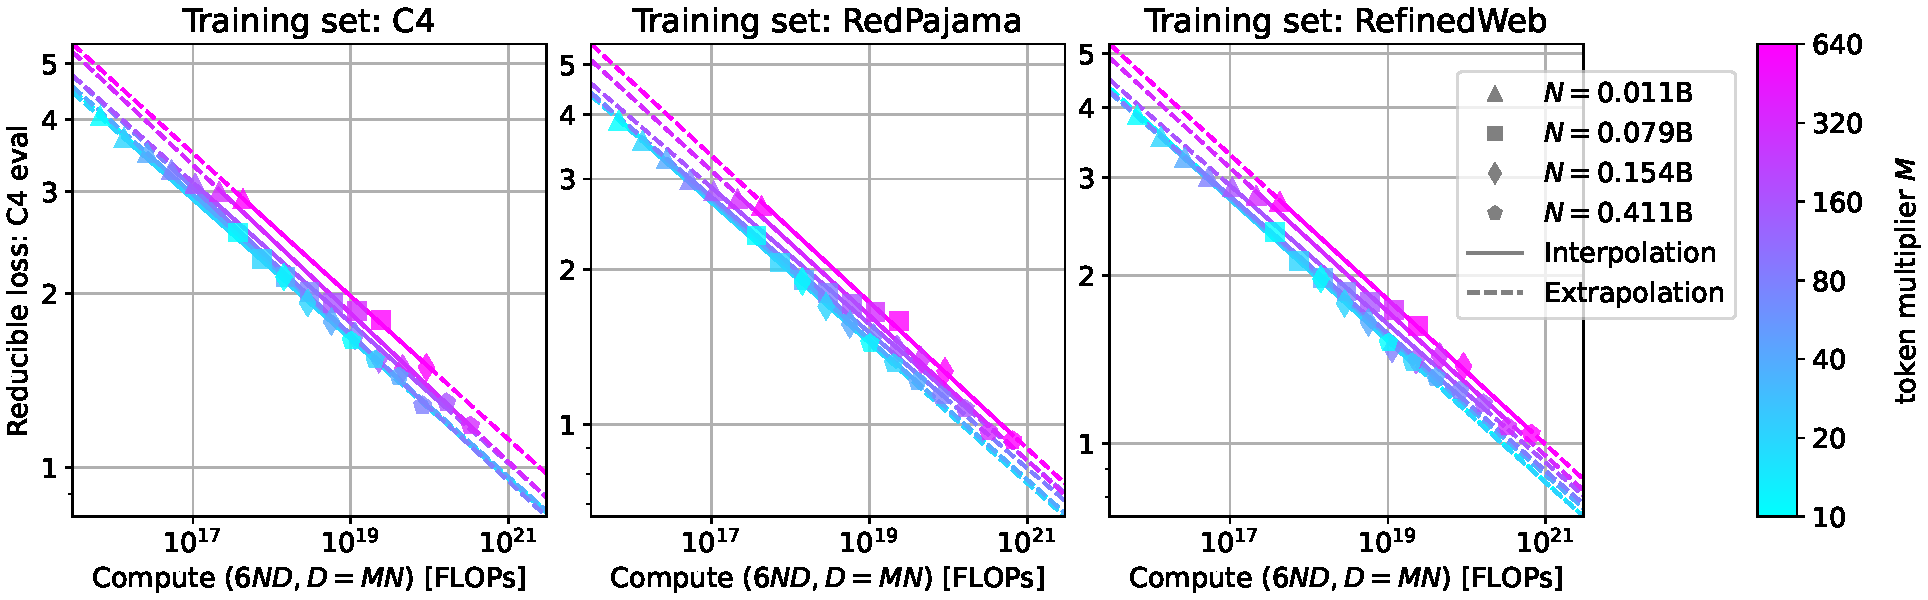
\includegraphics[width=0.98\linewidth]{figs/emperical.pdf}
    \caption{\textbf{Scaling in the over-trained regime follows consistent power law exponents.} We notice parallel lines in the $\log$-$\log$ plots of reducible loss vs. training compute for a range of token multipliers $M$, which give the ratio of training tokens to model parameters. Larger $M$ corresponds to more over-training.
    For a power law giving reducible loss as a function of compute: $L'(C) = \lambda \cdot C^{-\eta}$, the exponent $\eta$ remains relatively constant resulting in lines with approximately fixed slope (Figure~\ref{fig:slopes}).
    The scalar $\lambda$ that determines the $y$-intercept, however, shifts with different token multipliers.
    This suggests $\lambda$ is a function of the token multiplier, while $\eta$ is not.
    }
    \label{fig:emperical}
    % \vspace*{-4mm}
\end{figure*}


\subsection{Scaling laws for over-training}
\label{sec:method_overtraining}

To propose a scaling law for over-trained models, we first turn to empirical observation.
We train four model configurations with parameter counts between 0.011B and 0.411B for token multipliers $M$ between 20 and 640, where $M=20$ points lie roughly on the compute-optimal frontier, and larger $M$ corresponds to more over-training.
We defer experimental details to Section~\ref{sec:experiments} to focus on our observations first.
In Figure~\ref{fig:emperical}, we show loss against compute in a $\log$-$\log$ plot for the models trained on three datasets and evaluated on the C4 eval set. 
We notice parallel lines when fitting power laws to the reducible loss, which suggests a near-constant scaling exponent even with increased over-training. 
This indicates that scaling behavior should be describable in the amount of over-training.

In search of an analytic expression for the observations in Figure~\ref{fig:emperical}, we consider existing scaling literature.
A common functional form for the risk of a model, as proposed in prior work~\cite{rosenfeld_ConstructivePredictionGeneralization_2020,chinchilla} is,
\begin{align}
\label{eq:riskform}
L(N,D) = E + A N^{-\alpha} + B D^{-\beta}.
\end{align}
Recall from Section~\ref{sec:def}, $N$ is the number of parameters and $D$ the number of training tokens.
The constants $E, A, \alpha, B, \beta$ are fit from data.
By fitting this parametric form, \citet{chinchilla} find that scaling exponents $\alpha$ and $\beta$ are roughly equal, suggesting that one should scale $N$ and $D$ equally as compute increases. Hence, we assume $\alpha=\beta$. 
With this assumption, we reparameterize Equation~\eqref{eq:riskform} in terms of compute $C = 6ND$ and a token multiplier $M = D/N$. 
We get,
\begin{align}
\label{eq:lossCM}
L(C,M)
=
E + \left(a M^{\eta} + b M^{-\eta} \right) C^{-\eta},
\end{align}
where $\eta = \alpha/2$, $a = A(1/6)^{-\eta}$, $b=B(1/6)^{-\eta}$ gives the relation to Equation~\eqref{eq:riskform}.
For a complete derivation, see Appendix~\ref{appx:theory}.

Equation~\eqref{eq:lossCM} has the following interpretation:
(i) The scaling exponent $\eta$ is not dependent on $M$. Thus, we always expect lines with the same slope in the $\log$-$\log$ plot---as in Figure~\ref{fig:emperical}.  
(ii) The term $a M^{\eta} + b M^{-\eta}$ determines the offsets between curves with different token multipliers. Hence, we expect non-overlapping, parallel lines in the $\log$-$\log$ plot for the range of $M$ we consider---also consistent with Figure~\ref{fig:emperical}.

Recall that we make the assumption $\alpha=\beta$, which implies equal scaling of parameters and tokens as more compute is available. 
However, as explained in Appendix~\ref{appx:theory}, even if $\alpha\neq \beta$, we get a parameterization that implies the power-law exponent remains constant with over-training.


\begin{figure}[tp]
    \centering
    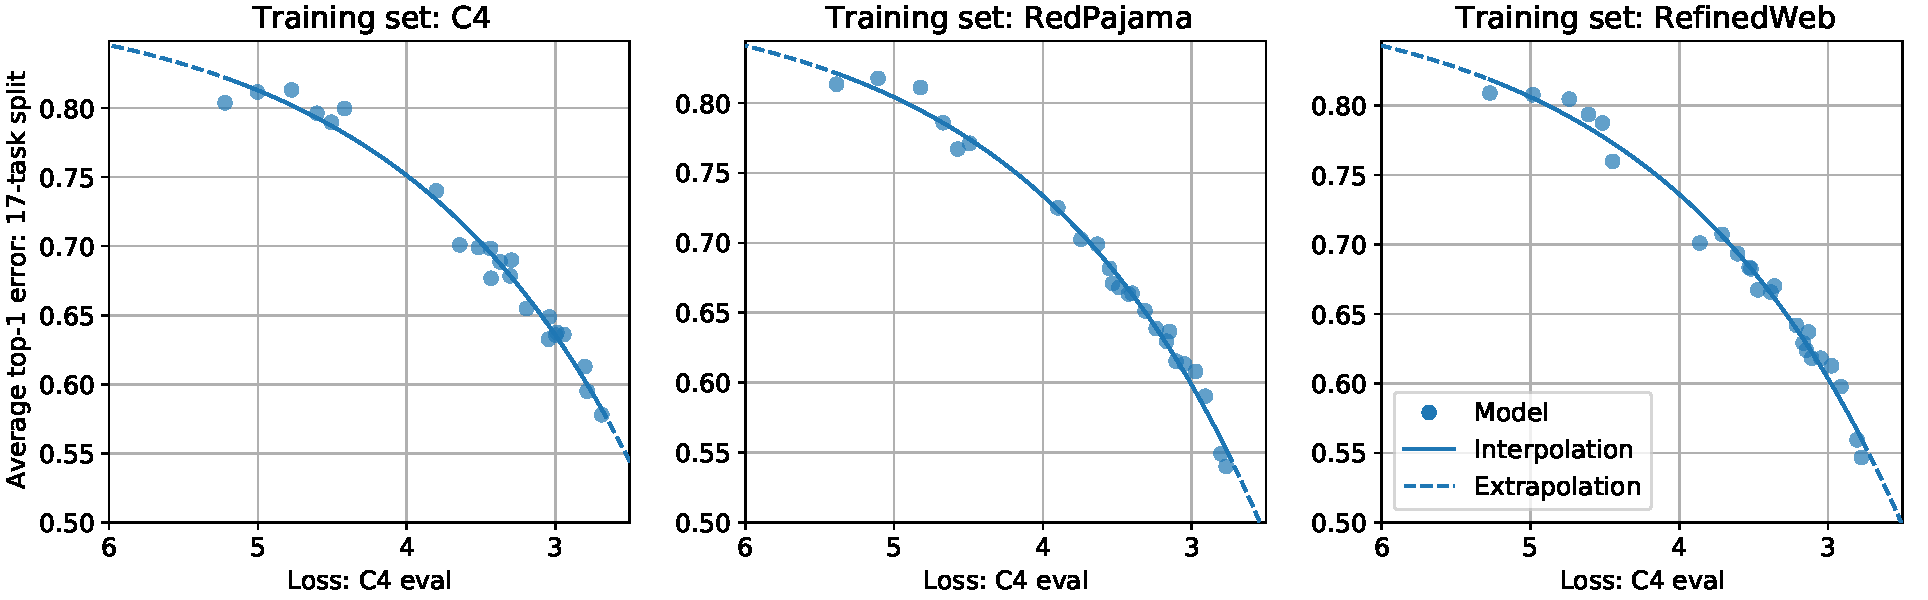
\includegraphics[width=0.98\linewidth]{figs/downstream_emperical.pdf}
    \caption{\textbf{Average top-1 error scales as a function of loss.} We plot models trained on three datasets and notice an exponential decay of average top-1 error as C4 eval loss, on the x-axis, decreases.
    We consider on the y-axes average error on 17 evaluations where performance is at least 10 points above random chance for at least one 0.154B scale model.
    These observations suggest that average top-1 error should be predictable with reliable loss estimates.
    }
    \label{fig:downstream_corr}
    % \vspace*{-3mm}
\end{figure}

\subsection{Scaling laws for downstream error}
\label{sec:method_downstream}

Scaling is typically studied in the context of loss~\cite{kaplan2020scaling,chinchilla,muennighoff2023scaling}, which \citet{schaeffer2023emergent} note is smoother than metrics like accuracy.
However, practitioners often use downstream benchmark accuracy as a proxy for model quality and not loss on perplexity evaluation sets.
To better connect scaling laws and over-training to task prediction, we revisit the suite of models plotted in Figure~\ref{fig:emperical}.
In Figure~\ref{fig:downstream_corr}, we plot average downstream top-1 errors over evaluations sourced from LLM-Foundry~\cite{mosaicml} against the C4 eval loss.
We defer details of the setup to Section~\ref{sec:experiments} to focus here on a key observation: average error appears to follow exponential decay as loss decreases.

Based on the exponential decay we observe in Figure~\ref{fig:downstream_corr}, we propose the following relationship between downstream average top-1 error \textsf{Err} and loss $L$,
\begin{align}
\label{eq:errL}
\textsf{Err}(L) = \epsilon - k \cdot \exp{(-\gamma L)},
\end{align}
where $\epsilon, k, \gamma$ are fit from data.
Equation~\eqref{eq:errL} also has an interpretation in terms of model perplexity $\textsf{PP}(L) = \exp{(L})$,
\begin{align}
\label{eq:errPP}
\textsf{Err}(\textsf{PP}) = \epsilon - k \cdot \textsf{PP}^{-\gamma}.
\end{align}
Namely, \textsf{Err} follows a power law in $\textsf{PP}$ that is bounded from above by $\epsilon$ signifying arbitrarily high error and from below by $\epsilon - k \cdot 
\exp(-\gamma E)$, where $E$ is the Bayes error from Equation~\eqref{eq:lossCM}.

Equation~\eqref{eq:errL} in conjunction with Equation~\eqref{eq:lossCM} suggests a three-step method to predict $\textsf{Err}$ as a function of compute and the amount of over-training.
For choices of training and validation distributions,
(i) fit a scaling law to Equation~\eqref{eq:lossCM} using triplets of compute $C$, token multiplier $M$, and measured loss $L$ on a validation set to yield $(C, M) \mapsto L$.
(ii) Fit a scaling law to Equation~\eqref{eq:errL}  using pairs of loss $L$ and downstream error $\textsf{Err}$ for models to get $L \mapsto \textsf{Err}$.
(iii) Chain predictions to get $(C, M) \mapsto \textsf{Err}$.